\documentclass{article}

\newcommand{\bra}[1]{\left(#1\right)}
\usepackage[activate={true,nocompatibility},final,tracking=true,kerning=true,spacing=true,factor=1100,stretch=10,shrink=10]{microtype}
\microtypecontext{spacing=nonfrench}
\usepackage{tikz}
\usepackage{tikz-cd}
\usepackage{mathpazo}
\usepackage{amsmath,amsthm,amssymb}
\usepackage{subcaption}
\usepackage{enumerate}
\usetikzlibrary{shapes}
\usetikzlibrary{positioning}
\usetikzlibrary{decorations.pathmorphing}
% Set up the images/graphics package
\usepackage{graphicx,float}
\setkeys{Gin}{width=\linewidth,totalheight=\textheight,keepaspectratio}
\graphicspath{{.}}
\usepackage{hyperref}
\hypersetup
{
  colorlinks=true,
  linkcolor=blue!50!black!100,
  filecolor=blue,      
  urlcolor=blue,
  citecolor=blue
}

% Small sections of multiple columns
\usepackage{multicol}
\usepackage[margin=1.6in]{geometry}

%--------Theorem Environments--------
%theoremstyle{plain} --- default
\newtheorem{thm}{Theorem}
\newtheorem{cor}[thm]{Corollary}
\newtheorem{prop}[thm]{Proposition}
\newtheorem{lem}[thm]{Lemma}
\newtheorem{fact}[thm]{Fact}
\newtheorem{conj}[thm]{Conjecture}
\newtheorem{quest}[thm]{Question}
\newtheorem{claim}{Claim}

\theoremstyle{definition}
\newtheorem{defn}[thm]{Definition}
\newtheorem{defns}[thm]{Definitions}
\newtheorem{con}[thm]{Construction}
\newtheorem{exmp}[thm]{Example}
\newtheorem{jk}[thm]{Joke}
\newtheorem{exmps}[thm]{Examples}
\newtheorem{notn}[thm]{Notation}
\newtheorem{notns}[thm]{Notations}
\newtheorem{addm}[thm]{Addendum}
\newtheorem{exer}[thm]{Exercise}

\theoremstyle{remark}
\newtheorem{rem}[thm]{Remark}
\newtheorem{ans}[thm]{Answer}
\newtheorem{rems}[thm]{Remarks}
\newtheorem{warn}[thm]{Warning}
\newtheorem{sch}[thm]{Scholium}

% MACROS
\newcommand{\Mod}[1]{\ (\text{mod}\ #1)}
\newcommand{\R}{\mathbb{R}}
\newcommand{\N}{\mathbb{N}}
\newcommand{\Q}{\mathbb{Q}}
\newcommand{\F}{\mathbb{F}}
\newcommand{\Z}{\mathbb{Z}}
\newcommand{\mC}{\mathcal{C}}
\newcommand{\mG}{\mathcal{G}}
\newcommand{\mP}{\mathcal{P}}
\newcommand{\one}{\mathbb{1}}
\renewcommand{\P}{\mathbb{P}}
\DeclareMathOperator{\dist}{dist}
\DeclareMathOperator{\aut}{Aut}
\DeclareMathOperator{\gal}{Gal}
\DeclareMathOperator{\orb}{Orb}
\DeclareMathOperator{\stab}{Stab}
\DeclareMathOperator{\inn}{Inn}
\DeclareMathOperator{\spn}{Span}
\DeclareMathOperator{\out}{Out}
\DeclareMathOperator{\im}{Im}
\DeclareMathOperator{\arr}{Arr}
\DeclareMathOperator{\rk}{rk}
\DeclareMathOperator{\rcf}{rcf}
\DeclareMathOperator{\tors}{Tors}
\DeclareMathOperator{\Hom}{Hom}
\DeclareMathOperator{\ann}{Ann}
\DeclareMathOperator{\Alg}{Alg}
\newcommand{\norm}[1]{\left\lVert #1 \right\rVert}
\newcommand{\inp}[2]{\left\langle #1, #2 \right\rangle}
\newcommand{\id}{\mathrm{id}}
\newcommand{\gln}{\text{GL}_n}
\newcommand{\op}[1]{#1^{\text{op}}}
\newcommand{\pullback}{\mbox{\LARGE$\lrcorner$}}
\newcommand{\pushout}{\mbox{\LARGE$\ulcorner$}}
\newcommand{\inl}{\textsf{inl}}
\newcommand{\inr}{\textsf{inr}}
\newcommand{\mPne}{\mathcal{P}_{\text{ne}}}
\newcommand{\Carr}{\mathcal{C}^{\downarrow}}

\title{Episode 8 - Monads and Algebras\vspace{-10pt}}
\author{Ralph Sarkis}
\date{\vspace{-10pt}\today\vspace{-15pt}}  % if the \date{} command is left out, the current date will be used
\begin{document}
\maketitle
\begin{abstract}
    We introduce monads from three point of views: categorical, algebraic and computational.
\end{abstract}
\section{POV: Category Theory}
%Composition of adjunctions
We will start from the concept of an adjunction which, as we hope was made clear in the previous lecture, is ubiquitous and powerful throughout mathematics. However, we will start with a great oversimplification; we will assume the categories concerned are posetal.

An adjunction between posets is more commonly called a Galois connection.
\begin{defn}[Galois connection]
    Let $(P, \leq)$ and $(Q, \sqsubseteq)$ be posets. A \textbf{Galois connection} between them is a pair of order-preserving functions $L: P \rightarrow Q$ and $R: Q \rightarrow P$ satisfying for any $p \in P$ and $q \in Q$, $L(p) \sqsubseteq q \iff p \leq R(q)$. 
\end{defn}
We are now interested in the composition $R\circ L$. It is also a monotonic function but the results about adjoints we have seen yield a couple of interesting properties. First, the existence of the unit $\eta: \id_P \Rightarrow RL$ means that for any $p \in P$, there is $\eta_p : p \rightarrow RL(p)$, so $RL$ is \textbf{extensive} (i.e.: $\forall p\in P, p\leq RL(p)$). Second, the existence of the counit $\varepsilon: RL \Rightarrow \id_P$ means that for any $p \in P$, there is $R(\varepsilon_{L(p)}) : RLRL(p) \rightarrow RL(p)$ and $RL(\eta_p): RL(p) \rightarrow RLRL(p)$, so $RL$ is idempotent (i.e.: $\forall p \in P, RL(p) = RLRL(p)$). We say that $RL$ is a closure operator.
%Closure operator
\begin{defn}[Closure operator]
    Let $(P, \leq)$ be a poset, a \textbf{closure operator} on $P$ is a monotone extensive and idempotent function $c: P \rightarrow P$.
\end{defn}
\begin{exmp}
    We can give a very simple example hinting at the origins of the terminology. Consider the real numbers $\R$ with the standard topology. We know that $(\mathcal{P}(\R), \subseteq)$ is a poset and we can define $c: \mathcal{P}(\R) \rightarrow \mathcal{P}(\R)$ sending $U\subseteq \R$ to its closure $c(U)$ in the topological sense as in $c(U)$ is the set of limit points of $U$. Then, you probably have seen that for any $U,V\subseteq \R$, $U\subseteq V \implies c(U) \subseteq c(V)$, $U \subseteq c(U)$ and $c(U) = c(c(U))$, thus operation of closure is a closure operator.
\end{exmp}

We will generalize this discussion to arbitrary categories now. Let $L:\begin{tikzcd}[cramped,sep=small]
	{\mathbf{C}} & {\mathbf{D}}
	\arrow[from=1-1, to=1-2, shift left=1]
	\arrow[from=1-2, to=1-1, shift left=1]
\end{tikzcd}:R$ be an adjoint pair of functors, we have two natural transformations $\eta: \id_{\mathbf{C}} \Rightarrow RL$ and $R\varepsilon L : RLRL \Rightarrow RL$. Recall these may interact well together via the zig-zag identities that we reformulate in \eqref{diag-zigzagL} and \eqref{diag-zigzagR} and we add to those the commutativity diagram \eqref{diag-multadj} in the definition of $\varepsilon \diamond \varepsilon$.\\
\begin{minipage}{0.33\textwidth}
    \begin{equation}\label{diag-zigzagL}% https://q.uiver.app/?q=WzAsMyxbMCwwLCJMIl0sWzEsMCwiTFJMIl0sWzEsMSwiTCJdLFswLDEsIkxcXGV0YSIsMCx7ImxldmVsIjoyfV0sWzEsMiwiXFx2YXJlcHNpbG9uIEwiLDAseyJsZXZlbCI6Mn1dLFswLDIsIlxcb25lX0wiLDIseyJsZXZlbCI6Mn1dXQ==
        \begin{tikzcd}
            {L} & {LRL} \\
            & {L}
            \arrow[Rightarrow, "{L\eta}", from=1-1, to=1-2]
            \arrow[Rightarrow, "{\varepsilon L}", from=1-2, to=2-2]
            \arrow[Rightarrow, "{\one_L}"', from=1-1, to=2-2]
        \end{tikzcd}
    \end{equation}
\end{minipage}
\begin{minipage}{0.33\textwidth}
    \begin{equation}\label{diag-zigzagR}% https://q.uiver.app/?q=WzAsMyxbMSwwLCJSIl0sWzAsMCwiUkxSIl0sWzAsMSwiTCJdLFswLDEsIlxcZXRhIFIiLDIseyJsZXZlbCI6Mn1dLFsxLDIsIlJcXHZhcmVwc2lsb24iLDIseyJsZXZlbCI6Mn1dLFswLDIsIlxcb25lX0wiLDAseyJsZXZlbCI6Mn1dXQ==
        \begin{tikzcd}
            {RLR} & {R} \\
            {L}
            \arrow[Rightarrow, "{\eta R}"', from=1-2, to=1-1]
            \arrow[Rightarrow, "{R\varepsilon}"', from=1-1, to=2-1]
            \arrow[Rightarrow, "{\one_L}", from=1-2, to=2-1]
        \end{tikzcd}
    \end{equation}
\end{minipage}
\begin{minipage}{0.33\textwidth}
    \begin{equation}\label{diag-multadj}% https://q.uiver.app/?q=WzAsNCxbMCwwLCJMUkxSIl0sWzEsMCwiTFIiXSxbMSwxLCJcXGlkX0QiXSxbMCwxLCJMUiJdLFswLDEsIlxcdmFyZXBzaWxvbiBMUiIsMCx7ImxldmVsIjoyfV0sWzEsMiwiXFx2YXJlcHNpbG9uIiwwLHsibGV2ZWwiOjJ9XSxbMCwzLCJMUlxcdmFyZXBzaWxvbiIsMix7ImxldmVsIjoyfV0sWzMsMiwiXFx2YXJlcHNpbG9uIiwyLHsibGV2ZWwiOjJ9XV0=
        \begin{tikzcd}
            {LRLR} & {LR} \\
            {LR} & {\id_D}
            \arrow[Rightarrow, "{\varepsilon LR}", from=1-1, to=1-2]
            \arrow[Rightarrow, "{\varepsilon}", from=1-2, to=2-2]
            \arrow[Rightarrow, "{LR\varepsilon}"', from=1-1, to=2-1]
            \arrow[Rightarrow, "{\varepsilon}"', from=2-1, to=2-2]
        \end{tikzcd}
    \end{equation}
\end{minipage}\\
With a bit of tinkering, we can make these diagrams all about the functor we are interested in, namely $RL$. Indeed, if we denote $M = RL$ and $\mu = R\varepsilon L$ before acting by $R$ on the right of \eqref{diag-zigzagL}, $L$ on the left of \eqref{diag-zigzagR} and $R(\cdot)L$ on \eqref{diag-multadj}, we obtain the definition of a monad.  
%Def
\begin{defn}[Monad]
    A \textbf{monad} is a triple comprised of an endofunctor $M: \mathbf{C} \rightsquigarrow \mathbf{C}$ and two natural transformations $\eta: \id_{\mathbf{C}}\Rightarrow M$ and $\mu: M^2 \Rightarrow M$ called the \textbf{unit} and \textbf{multiplication} respectively that make \eqref{diag-unitmonad} and \eqref{diag-multmonad} commute in $[\mathbf{C},\mathbf{C}]$.\\
    \begin{minipage}{0.48\textwidth}
        \begin{equation}\label{diag-unitmonad}
            \begin{tikzcd}
                M \arrow[rd, Rightarrow, "\one_M"'] \arrow[r, Rightarrow, "M\eta"] & M^2 \arrow[d, Rightarrow, "\mu"] & M \arrow[ld, Rightarrow, "\one_M"] \arrow[l, Rightarrow, "\eta M"'] \\ & M &
            \end{tikzcd}
        \end{equation}
    \end{minipage}
    \begin{minipage}{0.48\textwidth}
        \begin{equation}\label{diag-multmonad}
            \begin{tikzcd}
                M^3 \arrow[d, Rightarrow, "\mu M"'] \arrow[r, Rightarrow, "M\mu"] & M^2 \arrow[d, Rightarrow, "\mu"] \\
                M^2 \arrow[r, Rightarrow, "\mu"'] & M
            \end{tikzcd}
        \end{equation}
    \end{minipage}
\end{defn}
\begin{exmps}\label{exmp-monads}
    Our discussion above tells us that any adjoint pair $L\dashv R$ corresponds to a monad $(RL, \eta, R\varepsilon L)$, so all the examples of adjunctions you have seen correspond to suitable examples of monads. For instance, all closure operators are monads. Here, we describe three simple yet very useful examples and let you ponder on the adjunctions they might or might not originate from.
    \begin{enumerate}
        \item Suppose $\mathbf{C}$ has (binary) coproducts and a terminal object $\mathbf{1}$, then $(\cdot + \mathbf{1}): \mathbf{C} \rightsquigarrow \mathbf{C}$ is a monad. We write $\inl^{X+Y}$ (resp. $\inr^{X+Y}$) for the injection of $X$ (resp. $Y$) into $X+Y$. First, note that for a morphism $f: X \rightarrow Y$, \[f+\mathbf{1} = [\inl^{Y+\mathbf{1}} \circ f, \inr^{Y+\mathbf{1}}]: X+ \mathbf{1} \rightarrow Y + \mathbf{1}.\]
        The components of the unit are given by the coprojections, i.e.: $\eta_X = \inl^{X+\mathbf{1}} : X \rightarrow X+ \mathbf{1}$, and the components of the multiplication are \[\mu_X = [\inl^{X+\mathbf{1}}, \inr^{X+\mathbf{1}}, \inr^{X+\mathbf{1}}]: X+ \mathbf{1} + \mathbf{1} \rightarrow X + \mathbf{1}.\]
        Checking that \eqref{diag-unitmonad} commutes, we have for any $X \in \mathbf{C}$:%TODO: justifications
        \begin{align*}
            \mu_X \circ (\eta_X+\mathbf{1}) &= [\mu_X \circ \inl^{(X+\mathbf{1})+\mathbf{1}} \circ \eta_X, \mu_X \circ \inr^{(X+\mathbf{1})+\mathbf{1}}]\\
            &= [[\inl^{X+\mathbf{1}}, \inr^{X+\mathbf{1}}] \circ \inl^{X+\mathbf{1}}, \inr^{X+\mathbf{1}}]\\
            &= [\inl^{X+\mathbf{1}}, \inr^{X+\mathbf{1}}]\\
            &= \id_{X+\mathbf{1}}\\
            &= [\inl^{X+\mathbf{1}}, \inr^{X+\mathbf{1}}]\\
            &= \mu_X \circ \inl^{(X+\mathbf{1})+\mathbf{1}}\\
            &= \mu_X \circ \eta_{X+\mathbf{1}}
        \end{align*}
        For \eqref{diag-multmonad}, we have for any $X\in \mathbf{C}$: %TODO: justifications.
        \begin{align*}
            \mu_X \circ (\mu_X+\mathbf{1}) &= [\mu_X \circ \inl^{(X+\mathbf{1})+\mathbf{1}} \circ \mu_X, \mu_X \circ \inr^{(X+\mathbf{1})+\mathbf{1}}]\\
            &= [[\inl^{X+\mathbf{1}}, \inr^{X+\mathbf{1}}] \circ \mu_X, \inr^{X+\mathbf{1}}]\\
            &= [[\inl^{X+\mathbf{1}}, \inr^{X+\mathbf{1}}, \inr^{X+\mathbf{1}}], \inr^{X+\mathbf{1}}]\\
            &= [\mu_X, \inr^{X+\mathbf{1}}]\\
            &= [[\inl^{X+\mathbf{1}}, \inr^{X+\mathbf{1}}], \inr^{X+\mathbf{1}}, \inr^{X+\mathbf{1}}]\\
            &= [\mu_X \circ \inl^{(X+\mathbf{1})+\mathbf{1}}, \mu_X \circ \inr^{(X+\mathbf{1})+\mathbf{1}}, \mu_X \circ \inr^{(X+\mathbf{1})+\mathbf{1}}]\\
            &= \mu_X \circ \mu_{X+\mathbf{1}}
        \end{align*}
        \item The covariant powerset functor $\mP:\textbf{Set}\rightsquigarrow \textbf{Set}$ is a monad with the following unit and multiplication:
        \[ \eta_X: X \rightarrow \mP(X) = x \mapsto \{x\} \text{ and } \mu_X: \mP(\mP(X)) \rightarrow \mP(X) = F \mapsto \bigcup_{s \in F} s.\]
        Checking that \eqref{diag-unitmonad}, we have for any $S \subseteq \mP(X)$,
        \begin{align*}
            \mu_X(\mP(\eta_X)(S)) &= \mu_X\left( \{\{x\} \mid x \in S\} \right)\\
            &= \bigcup_{x \in S} \{x\}\\
            &= S\\
            &= \bigcup\{S\}\\
            &= \mu_X(\{S\})\\
            &= \mu_X(\eta_{\mP(X)}(S))
        \end{align*}
        Checking that \eqref{diag-multmonad} commutes, we have for any $\mathcal{F} \in \mP(\mP(\mP(X))$,
        \begin{align*}
            \mu_X(\mu_{\mP(X)}(\mathcal{F})) &= \mu_X\left( \bigcup_{F \in \mathcal{F}} F \right)\\
            &= \bigcup_{\substack{s\in \mP(X)\\\exists F \in \mathcal{F}, s \in F}} s\\
            &= \left\{ x \in X \mid \exists s \in \mP(X), x \in s \text{ and } \exists F \in \mathcal{F}, s \in F\right\}\\
            &= \bigcup_{F \in \mathcal{F}}\bigcup_{s \in F} s\\
            &= \mu_X\left( \left\{ \bigcup_{s \in F} s \mid F \in \mathcal{F}\right\} \right)\\
            &= \mu_X(\mP(\mu_X)(\mathcal{F}))
        \end{align*}
        \item\label{exmp-distmonad} The functor $\mathcal{D}: \textbf{Set} \rightarrow \textbf{Set}$ sends a set $X$ to the set of finitely supported distributions on $X$, i.e.:
        \[\mathcal{D}(X) := \{\varphi \in [0,1]^X \mid \sum_{x \in X} \varphi(x) = 1 \text{ and } \varphi(x) \neq 0 \text{ for finitely many $x$'s}\}.\]
        It sends a function $f: X \rightarrow Y$ to the function between distributions \[\lambda \varphi^{\mathcal{D}(X)}. \lambda y^{Y}. \varphi(f^{-1}(y)).\]
        More verbosely, the weight of $\mathcal{D}(f)(\varphi)$ at point $y$ is equal to the total weight of $\varphi$ on the preimage of $y$ under $f$. It is a monad with unit $\eta_X = x \mapsto \delta_x$, where $\delta_x$ is the Dirac distribution at $x$ (all the weight is at $x$), and multiplication 
        \[\mu_X = \Phi \mapsto \lambda x^X. \sum_{\phi \in \text{supp}(\Phi)} \Phi(\phi) \cdot \phi(x),\]
        where $\text{supp}(\Phi)$ is the support of $\Phi$, i.e.: $\text{supp}(\Phi) := \{\varphi \mid \Phi(\varphi) \neq 0\}$. 
    \end{enumerate}
\end{exmps}

%Monad -> adjunctions
After looking long enough for adjunctions giving rise to the monads in Example \ref{exmp-monads}, two questions dare to be asked. Does every monad arise from an adjunction? If yes, is that adjunction unique?

The second question might not be as natural to novices in category theory but it is almost as important as the first one. Indeed, uniqueness is a very strong property and if every monad had a unique corresponding adjunction, one might expect it to be fairly easy to find. This is part of the beauty of category theory. We are working with very little data $M$, $\eta$ and $\mu$ so if it completely determined an adjunction $L$, $R$ and $\Hom(L(-), -) \cong \Hom(-,R(-))$, it could not do so in a very convoluted way merely because there is not that many ways to manipulated the original data.

In any case, we will respectively give a positive and negative answer to these questions. Fortunately, while we might not benefit from the power of uniqueness, there are two special adjunctions arising from a monad whose descriptions are fairly straightforward. In the order we present them, the first is due to Kleisli and the second to Eilenberg and Moore. In the rest of this section, $(M, \eta, \mu)$ will be a monad on a category $\mathbf{C}$.
\subsection{Kleisli Category $\mathbf{C}_M$}
An intuitive way to think about monads is through \textit{generalized elements}. Given an object $A \in \mathbf{C}_0$, we can view $MA$ as extending $A$ with more general or structured elements built from $A$.

In this picture, the morphisms $\eta_A: A \rightarrow MA$ give a way to understand anything inside $A$ trivially as a general element of $A$. The morphisms $\mu_A : M^2A \rightarrow MA$ imply that higher order structures can collapsed so that generalized elements over generalized elements of $A$ are generalized elements of $A$. The functoriality of $M$ implies that the new structures in $MA$ are somewhat independent of $A$. Indeed, for every morphisms $f: A \rightarrow B$, there is a morphism $Mf: MA \rightarrow MB$ which, by naturality of $\eta$ ($Mf(\eta_A(-)) = \eta_B(f(-))$), acts just like $f$ on the trivial generalization of elements in $A$. Commutativity of \eqref{diag-unitmonad} says that the trivial generalization (there are two ways to do it) of a generalized element is indeed trivial as after collapsing via $\mu$, we end up with what we started with. Finally, the associativity of $\mu$ (i.e.: commutativity of \eqref{diag-multmonad}) corresponds to the fact that in higher order of generalizations, one can collapse the structure at every level in any order and end up with the same thing.

Now, we can also consider \textit{generalized morphisms}. Let us say we were given an ill-defined morphism $f: A \rightarrow B$ that sends some of the stuff in $A$ outside of $B$. One way to fix this might be to consider general elements of $B$ and see $f$ as a morphism $A \rightarrow MB$. We will call such morphisms \textbf{Kleisli morphisms} and write $f:A \rightarrow MB$ or $f: A \nrightarrow B$.

With an arbitrary functor $F$, you might have a hard time to come up with a way to compose them Kleisli morphisms $A \rightarrow FB$ and $B \rightarrow FC$ or define the identity Kleisli morphism $A \rightarrow FA$, but the data of a monad lets you do just that. We end up with the category $\mathbf{C}_M$.
\begin{defn}[$\mathbf{C}_M$]
    Let $\mathbf{C}$ be a category and $(M,\eta, \mu)$ a monad on $\mathbf{C}$. The \textbf{Kleisli category} of $M$, denoted $\mathbf{C}_M$ has objects $\mathbf{C}_0$ and morphisms $f: A \rightarrow MB \in \mathbf{C}_1$. The identity for $A$ is $\eta_A:A \rightarrow MA$ and composition is given by \[g \circ_M f = \mu_C \circ Mg \circ f: A \nrightarrow C,\] where $f: A \nrightarrow B$ and $g: B \nrightarrow C$.
\end{defn}
Checking that this is indeed a category is left as an exercise and you should remark that it requires using all the properties $M$, $\eta$ and $\mu$ satisfy.

As we have constructed $\mathbf{C}_M$ with objects and morphisms in $\mathbf{C}$, we would like to describe a forgetful functor $U_M: \mathbf{C}_M \rightsquigarrow \mathbf{C}$. A first guess to send objects $A$ to themselves will fail when it is time to defining the action of $U_M$ on morphisms for $f: A \nrightarrow B$ can send some stuff into generalized elements of $B$, and we have no way to get this back into $B$. Instead, we need to generalize everything before going into $\mathbf{C}$, namely, $U_M(A) = MA$ and $U_Mf = \mu_B \circ Mf : MA \rightarrow MB$.

We can check that for any $A$, $U_M(\eta_A) = \mu_A \circ M(\eta_A) \stackrel{\eqref{diag-unitmonad}}{=} \id_A$ and for any for any $f: A \nrightarrow B$ and $g: B \nrightarrow C$,
\begin{align*}
    U_M(g \circ_M f) &= U_M(\mu_C \circ Mg\circ f)\\
    &= \mu_C \circ M(\mu_C \circ Mg \circ f)\\
    &= \mu_C \circ M(\mu_C) \circ MMg \circ Mf\\
    &= \mu_C \circ \mu_{MC} \circ MMg \circ Mf &&\text{by \eqref{diag-multmonad}}\\
    &= \mu_C \circ Mg \circ \mu_B \circ Mf &&\text{by naturality of $\mu$}\\
    &= U_M(g) \circ U_M(f).
\end{align*}
We conclude that $U_M$ is a functor.

In the opposite direction, we want a functor $F_M: \mathbf{C} \rightsquigarrow \mathbf{C}_M$. This time, we send $A$ to itself because we can make any morphism $f: A \rightarrow B$ generalized by post-composing with $\eta_B$, namely $F_M(A) = A$ and $F_M(f) = \eta_B \circ f$ for any $f: A \rightarrow B$. For functoriality, $F_M(\id_A)$ is trivial as $\eta_A$ is the identity on $A$ in $\mathbf{C}_M$ and \begin{align*}
    F_M(g \circ f) &= \eta_C \circ g \circ f\\
    &= Mg \circ \eta_B \circ f&&\text{by naturality of $\eta$}\\
    &= Mg \circ \mu_B \circ M(\eta_B) \circ \eta_B \circ f&&\text{by \eqref{diag-unitmonad}}\\
    &= \mu_C \circ MMg \circ M(\eta_B) \circ \eta_B \circ f &&\text{by naturality of $\mu$}\\
    &= \mu_C \circ M(\eta_C) \circ Mg \circ \eta_B \circ f &&\text{by naturality of $\eta$}\\
    &= F_M(g) \circ_M F_M(f)
\end{align*}

Before checking that this is indeed an adjunction, we need to make sure it composes to $M$, that is $U_MF_M = M$. On objects, it is clear. On a morphism $f: A \rightarrow B$, we have 
\[U_M(F_M(f)) = U_M(\eta_B \circ f) = \mu_B \circ M(\eta_B) \circ Mf \stackrel{\eqref{diag-unitmonad}}{=} Mf.\]
Let us now verify that $F_M \dashv U_M$.
Let $A, B \in \mathbf{C}_0$ (we view $B$ as an object of $\mathbf{C}_M$), we need to exhibit a natural isomorphism $\Hom_{\mathbf{C}_M}(F_MA,B) \cong \Hom_{\mathbf{C}}(A,U_MB)$. The isomorphism is clear as $U_MB = MB$, $F_MA = A$ and a morphism $A \rightarrow MB$ is precisely a Kleisli morphism $A \nrightarrow B$, we will denote it $\id$. For the naturality, we need to show the following square commutes for any $f: A' \rightarrow A$ and $g: B \nrightarrow B'$.
\begin{equation}\label{diag-adjF_MU_M}
    % https://q.uiver.app/?q=WzAsNCxbMSwwLCJcXEhvbV97XFxtYXRoYmZ7Q319KEEsTUIpIl0sWzAsMCwiXFxIb21fe1xcbWF0aGJme0N9X019KEEsQikiXSxbMCwxLCJcXEhvbV97XFxtYXRoYmZ7Q31fTX0oQScsQicpIl0sWzEsMSwiXFxIb21fe1xcbWF0aGJme0N9fShBJyxNQicpIl0sWzEsMCwiXFxpZCJdLFsxLDIsImcgXFxjaXJjICgtKVxcY2lyY19NIEZfTWYiLDJdLFswLDMsIlVfTWcgXFxjaXJjICgtKVxcY2lyYyBmIl0sWzIsMywiXFxpZCIsMl1d
    \begin{tikzcd}
        {\Hom_{\mathbf{C}_M}(A,B)} & {\Hom_{\mathbf{C}}(A,MB)} \\
        {\Hom_{\mathbf{C}_M}(A',B')} & {\Hom_{\mathbf{C}}(A',MB')}
        \arrow["{\id}", from=1-1, to=1-2]
        \arrow["{g \circ_M (-)\circ_M F_Mf}"', from=1-1, to=2-1]
        \arrow["{U_Mg \circ (-)\circ f}", from=1-2, to=2-2]
        \arrow["{\id}"', from=2-1, to=2-2]
    \end{tikzcd}
\end{equation}
It follows from the following derivation starting with a morphism $k: A \rightarrow MB$.
\begin{align*}
    g \circ_M k \circ_M F_Mf &= \mu_{B'} \circ M(g) \circ \mu_B \circ M(k) \circ \eta_{A} \circ f\\
    &= \mu_{B'} \circ M(g) \circ \mu_B \circ \eta_{MB} \circ k \circ f &&\text{by naturality of $\eta$}\\
    &= \mu_{B'} \circ M(g) \circ \id_{MB} \circ k \circ f&&\text{by \eqref{diag-unitmonad}}\\
    &= \mu_{B'} \circ M(g) \circ k \circ f\\
    &= U_Mg \circ k \circ f
\end{align*}

Recall that we claimed $(F_M,U_M)$ was special in some way and that this was the (informal) reason why it was relatively easy to find, the next proposition will make this precise.
\begin{defn}[$\mathrm{Adj}_M$]
    Let $\mathbf{C}$ be a category and $(M,\eta, \mu)$ a monad on $\mathbf{C}$. The category of adjunctions inducing $M$ is denoted $\mathrm{Adj}_M$. Its objects are adjoint pairs $(L,R)$ with $R\circ L = M$ whose unit is $\eta$ and whose counit $\varepsilon$ satisfies $R\varepsilon L = \mu$. Its morphisms $(L,R) \rightarrow (L',R')$ are functors $K$ satisfying $K\circ L = L'$ and $R'\circ K = R$ as in \eqref{diag-morphadj}.
    \begin{equation}\label{diag-morphadj}
        % https://q.uiver.app/?q=WzAsMyxbMCwwLCJcXG1hdGhiZntEfSJdLFsyLDAsIlxcbWF0aGJme0R9JyJdLFsxLDEsIlxcbWF0aGJme0N9Il0sWzAsMSwiSyJdLFsyLDAsIkwiLDAseyJvZmZzZXQiOi0yfV0sWzIsMSwiTCciLDAseyJvZmZzZXQiOi0yfV0sWzAsMiwiUiIsMCx7Im9mZnNldCI6LTF9XSxbMSwyLCJSJyIsMCx7Im9mZnNldCI6LTJ9XSxbNCw2LCIiLDAseyJsZXZlbCI6MSwic3R5bGUiOnsibmFtZSI6ImFkanVuY3Rpb24ifX1dLFs1LDcsIiIsMix7ImxldmVsIjoxLCJzdHlsZSI6eyJuYW1lIjoiYWRqdW5jdGlvbiJ9fV1d
        \begin{tikzcd}
            {\mathbf{D}} && {\mathbf{D}'} \\
            & {\mathbf{C}}
            \arrow["{K}", from=1-1, to=1-3]
            \arrow["{L}"{name=0}, from=2-2, to=1-1, shift left=2]
            \arrow["{L'}"{name=1}, from=2-2, to=1-3, shift left=2]
            \arrow["{R}"{name=2}, from=1-1, to=2-2, shift left=2]
            \arrow["{R'}"{name=3}, from=1-3, to=2-2, shift left=2]
            \arrow["\dashv"{rotate=50}, from=0, to=2, phantom]
            \arrow["\dashv"{rotate=-50}, from=1, to=3, phantom]
        \end{tikzcd}
    \end{equation}
\end{defn}
Let us first check that $(F_M,U_M)$ induces $(M, \eta, \mu)$, we already know that $U_MF_M = M$, but it remains to find the unit and counit of this adjunction. We will need to use the correspondence between the definitions of adjoint pairs seen in the last lecture. Recall that the natural isomorphism $\Hom_{\mathbf{C}_M}(F_M-,-) \cong \Hom_{\mathbf{C}}(-,U_M-)$ is simply the identity function between these two sets. Hence, the unit of the adjunction is $\mathbf{C}_0 \ni A \mapsto \id(u_{\mathbf{C}_M}(F_MA)) = \eta_A$ and the counit is $(\mathbf{C}_M)_0 \ni A \mapsto \id(u_{\mathbf{C}}(U_MA)) =: \varepsilon_A$. Note that $\varepsilon_A$ has type $MA \nrightarrow B$. We check that $U_M(\varepsilon_{F_MA}) = \mu_A$:
\[U_M(\varepsilon_{F_MA}) = \mu_A \circ \varepsilon_{F_MA} = \mu_A \circ u_{\mathbf{C}}(MA) = \mu_A.\]
\begin{prop}\label{prop-initKleisli}
    The adjunction $(F_M,U_M)$ is initial in $\mathrm{Adj}_M$.
\end{prop}
\begin{proof}
    Let $\mathbf{C}:L \dashv R: \mathbf{D} \in \mathrm{Adj}_M$ with unit $\eta$ and counit $\varepsilon$, we claim there is a unique functor $K:\mathbf{C}_M \rightsquigarrow  \mathbf{D}$ satisfying $K\circ F_M = L$ and $R \circ K = U_M$ as in \eqref{diag-initC_M}.
    \begin{equation}\label{diag-initC_M}
        \begin{tikzcd}
            {\mathbf{C}_M} && {\mathbf{D}} \\
            & {\mathbf{C}}
            \arrow["{K}", dashed, from=1-1, to=1-3]
            \arrow["{F_M}"{name=0}, from=2-2, to=1-1, shift left=2]
            \arrow["{L}"{name=1}, from=2-2, to=1-3, shift left=2]
            \arrow["{U_M}"{name=2}, from=1-1, to=2-2, shift left=2]
            \arrow["{R}"{name=3}, from=1-3, to=2-2, shift left=2]
            \arrow["\dashv"{rotate=50}, from=0, to=2, phantom]
            \arrow["\dashv"{rotate=-50}, from=1, to=3, phantom]
        \end{tikzcd}
    \end{equation}
    On objects, $K$ is determined by $KA = KF_MA = LA$. To a morphism $f: A \nrightarrow B$, we need to assign a morphism in $Kf \in \Hom_{\mathbf{D}}(LA, LB)$. Denote $\Phi_{A,B}: \Hom_{\mathbf{C}_M}(F_MA,B) \cong \Hom_{\mathbf{C}}(A,U_MB)$ and $\Psi_{A,B}: \Hom_{\mathbf{D}}(LA,B) \cong \Hom_{\mathbf{C}}(A,RB)$ be given by the adjunctions $F_M \dashv U_M$ and $L \dashv R$ respectively. Using the fact that $RK = U_M$, we obtain the following commutative diagram.
    % https://q.uiver.app/?q=WzAsOCxbMCwwLCJcXEhvbV97XFxtYXRoYmZ7Q31fTX0oRl9NQSxBKSJdLFsxLDAsIlxcSG9tX3tcXG1hdGhiZntDfX0oQSxVX01BKSJdLFsyLDAsIlxcSG9tX3tcXG1hdGhiZntDfX0oQSxSTEEpIl0sWzMsMCwiXFxIb21fe1xcbWF0aGJme0R9fShMQSxMQSkiXSxbMywyLCJcXEhvbV97XFxtYXRoYmZ7RH19KExBLExCKSJdLFsyLDIsIlxcSG9tX3tcXG1hdGhiZntDfX0oQSxSTEIpIl0sWzEsMiwiXFxIb21fe1xcbWF0aGJme0N9fShBLFVfTUIpIl0sWzAsMiwiXFxIb21fe1xcbWF0aGJme0N9X019KEZfTUEsQikiXSxbMCwxLCJcXFBoaV97QSxBfSJdLFsxLDJdLFszLDIsIlxcUHNpX3tBLExBfSIsMl0sWzQsNSwiXFxQc2lfe0EsTEJ9Il0sWzYsNV0sWzcsNiwiXFxQaGlfe0EsQn0iLDJdLFswLDcsImZcXGNpcmMgKC0pIiwxXSxbMyw0LCJLZiBcXGNpcmMgKC0pIiwxXSxbMSw2LCJVX01mIFxcY2lyYyAoLSkiLDFdLFsyLDUsIlJLZiBcXGNpcmMgKC0pIiwxXV0=
    \[\begin{tikzcd}
        {\Hom_{\mathbf{C}_M}(F_MA,A)} & {\Hom_{\mathbf{C}}(A,U_MA)} & {\Hom_{\mathbf{C}}(A,RLA)} & {\Hom_{\mathbf{D}}(LA,LA)} \\
        \\
        {\Hom_{\mathbf{C}_M}(F_MA,B)} & {\Hom_{\mathbf{C}}(A,U_MB)} & {\Hom_{\mathbf{C}}(A,RLB)} & {\Hom_{\mathbf{D}}(LA,LB)}
        \arrow["{\Phi_{A,A}}", from=1-1, to=1-2]
        \arrow[from=1-2, equals, to=1-3]
        \arrow["{\Psi_{A,LA}}"', from=1-4, to=1-3]
        \arrow["{\Psi_{A,LB}}", from=3-4, to=3-3]
        \arrow[from=3-2, equals, to=3-3]
        \arrow["{\Phi_{A,B}}"', from=3-1, to=3-2]
        \arrow["{f\circ_M (-)}" description, from=1-1, to=3-1]
        \arrow["{Kf \circ (-)}" description, from=1-4, to=3-4]
        \arrow["{U_Mf \circ (-)}" description, from=1-2, to=3-2]
        \arrow["{RKf \circ (-)}" description, from=1-3, to=3-3]
    \end{tikzcd}\]
    Because these adjunctions both have the same unit, we have $\Phi_{A,A}(u_{\mathbf{C}_M}(F_MA)) = \eta_A = \Psi_{A,A}(u_{\mathbf{D}}(LA))$. Therefore, if we start with $\eta_A \in \Hom_{\mathbf{C}_M}(F_MA,A)$ and follow the diagram, we infer that $Kf = \Psi_{A,LB}^{-1}(\Phi_{A,B}(f))$. Using the fact that $\Phi_{A,B}(f) = f$ and $\Psi_{A,LB}^{-1}(f) = \varepsilon_{LB} \circ Lf$ (follow the proof of the Yoneda lemma), we end up with $Kf = \varepsilon_{LB} \circ Lf$ and we can verify it is indeed functorial.
    \[K(u_{\mathbf{C}_M}(A)) = K(\eta_A) = \varepsilon_{LB} \circ L(\eta_A) \stackrel{\text{zig-zag}}{=} \id_A \]
    \begin{align*}
        K(g \circ_M f) &= K(\mu_C \circ RLg\circ f)\\
        &= \varepsilon_{LC} \circ L(\mu_C) \circ LRLg\circ Lf\\
        &= \varepsilon_{LC} \circ LR\varepsilon_{LC} \circ LRLg \circ Lf &&\text{by hypothesis on $\varepsilon$}\\
        &= \varepsilon_{LC} \circ \varepsilon_{LRLC} \circ LRLg \circ Lf&&\text{by naturality of $\varepsilon$}\\
        &= \varepsilon_{LC} \circ Lg \circ \varepsilon_{LB} \circ Lf&&\text{by naturality of $\varepsilon$}\\
        &= Kg \circ Kf\\
    \end{align*}
\end{proof}
\subsection{Eilenberg-Moore Category $\mathbf{C}^M$}
For the second solution to the problem of finding an adjunction inducing a given monad, we look at the more structural side of monads.
%Eilenberg-Moore
%TODO: motivational paragraph.
\begin{defn}[$M$--algebra]
    Let $(M,\eta, \mu)$ be a monad, an \textbf{Eilenberg-Moore algebra} for $M$ or simply $M$--\textbf{algebra} is a pair $(A, \alpha)$ consisting of an object $A \in \mathbf{C}_0$ and morphism $\alpha : MA \rightarrow A$ such that \eqref{diag-algunit} and \eqref{diag-algmult} commute.\\
    \begin{minipage}{0.48\textwidth}
        \begin{equation}\label{diag-algunit}
            \begin{tikzcd}
                A \arrow[rd, "\id_A"'] \arrow[r, "\eta_A"] & MA \arrow[d, "\alpha"] \\ & A
            \end{tikzcd}
        \end{equation}
    \end{minipage}
    \begin{minipage}{0.48\textwidth}
        \begin{equation}\label{diag-algmult}
            \begin{tikzcd}
                M^2A \arrow[d, "M(\alpha)"'] \arrow[r, "\mu_A"] & MA \arrow[d, "\alpha"] \\
                MA \arrow[r, "\alpha"']  & A  
                \end{tikzcd}
        \end{equation}
    \end{minipage}
\end{defn}
We will often denote an $M$--algebra using only its underlying set or morphism.
\begin{defn}[$M$--algebra homomorphism]
    Given two $M$--algebras $(A, \alpha)$ and $(B, \beta)$, an $M$--algebra homomorphism $f: (A, \alpha) \rightarrow (B, \beta)$ is a morphism $h:A \rightarrow B$ making \eqref{diag-alghom} commute.
    \begin{equation}\label{diag-alghom}
        \begin{tikzcd}
            MA \arrow[d, "\alpha"'] \arrow[r, "Mh"] & MB \arrow[d, "\beta"] \\
            A \arrow[r, "h"'] & B
        \end{tikzcd}
    \end{equation}
\end{defn}
For a monad $M$, the category of $M$--algebras is called the \textbf{Eilenberg-Moore} category of $M$ and denoted $\mathbf{C}^M$, composition and identities are induced by the composition and identities in $\mathbf{C}$. Again, since $\mathbf{C}^M$ was built from objects and morphisms in $\mathbf{C}$, there is an obvious candidate for a forgetful functor $U^M: \mathbf{C}^M \rightsquigarrow \mathbf{C}$ sending an $M$--algebra $(A,\alpha)$ to its underlying object $A$ and a homomorphism to its underlying morphism. Next, we need a left adjoint to $U^M$, $F^M: \mathbf{C} \rightsquigarrow \mathbf{C}^M$. Since we want $U^MF^M = M$ to hold, $F^M$ must send $A\in \mathbf{C}_0$ to an $M$--algebra over $MA$ and $h \in \mathbf{C}_1$ to $Mh$. There is only one choice given to us by the data of $M$, that is, $F^MA= (MA, \mu_A)$ and it turns out naturality of $\mu_A$ yields 
\begin{equation}
    \begin{tikzcd}
        M^2A \arrow[d, "\mu_A"'] \arrow[r, "M^2h"] & M^2B \arrow[d, "\mu_B"] \\
        MA \arrow[r, "Mh"'] & MB
    \end{tikzcd},
\end{equation}
which implies $Mh$ is indeed an $M$--algbera homomorphism. Let us now show that $F^M \dashv U^M$ with unit $\eta$ and counit $\varepsilon$ satisfying $U^M\varepsilon F^M = \mu$.

We want to exhibit an isomorphism $\Hom_{\mathbf{C}^M}(\mu_A, \beta) \cong \Hom_{\mathbf{C}}(A,B)$ natural in $A$ and $\beta: MB \rightarrow B$. In the forward direction, we send $h:MA \rightarrow B$ to $h \circ \eta_A: A \rightarrow B$ which ensures the unit of this adjunction is $\eta$. In the backwards direction, we send $h:A \rightarrow B$ to $\beta \circ Mh$ which is a homomorphism by the following diagram where (a) commutes by naturality of $\mu$ and (b) by $\beta$ being an $M$--algebra.
\begin{equation}
    % https://q.uiver.app/?q=WzAsNixbMCwwLCJNXjJBIl0sWzEsMCwiTV4yQiJdLFsyLDAsIk1CIl0sWzIsMSwiQiJdLFsxLDEsIk1CIl0sWzAsMSwiTUEiXSxbMCwxLCJNXjJmIl0sWzEsMiwiTVxcYmV0YSJdLFsyLDMsIlxcYmV0YSJdLFsxLDQsIlxcbXVfQiJdLFs0LDMsIlxcYmV0YSIsMV0sWzAsNSwiXFxtdV9BIiwyXSxbNSw0LCJNZiIsMl0sWzAsNCwiXFx0ZXh0eygxKX0iLDEseyJzdHlsZSI6eyJib2R5Ijp7Im5hbWUiOiJub25lIn0sImhlYWQiOnsibmFtZSI6Im5vbmUifX19XSxbMSwzLCJcXHRleHR7KDIpfSIsMSx7InN0eWxlIjp7ImJvZHkiOnsibmFtZSI6Im5vbmUifSwiaGVhZCI6eyJuYW1lIjoibm9uZSJ9fX1dXQ==
\begin{tikzcd}
	{M^2A} & {M^2B} & {MB} \\
	{MA} & {MB} & {B}
	\arrow["{M^2h}", from=1-1, to=1-2]
	\arrow["{M\beta}", from=1-2, to=1-3]
	\arrow["{\beta}", from=1-3, to=2-3]
	\arrow["{\mu_B}", from=1-2, to=2-2]
	\arrow["{\beta}" description, from=2-2, to=2-3]
	\arrow["{\mu_A}"', from=1-1, to=2-1]
	\arrow["{Mh}"', from=2-1, to=2-2]
	\arrow["{\text{(a)}}" description, from=1-1, to=2-2, phantom, no head]
	\arrow["{\text{(b)}}" description, from=1-2, to=2-3, phantom, no head]
\end{tikzcd}
\end{equation}
One can easily check that these operations are inverses of each other. Next, we turn to naturality. Let $f: A' \rightarrow A\in \mathbf{C}_1$ and $g: (B,\beta) \rightarrow (B',\beta')\in \mathbf{C}^M_1$, we claim that \eqref{diag-natEMadj} commutes.
\begin{equation}\label{diag-natEMadj}
    % https://q.uiver.app/?q=WzAsNCxbMCwwLCJcXEhvbV97XFxtYXRoYmZ7Q31eTX0oXFxtdV9BLFxcYmV0YSkiXSxbMSwwLCJcXEhvbV97XFxtYXRoYmZ7Q319KEEsQikiXSxbMSwxLCJcXEhvbV97XFxtYXRoYmZ7Q319KEEnLEInKSJdLFswLDEsIlxcSG9tX3tcXG1hdGhiZntDfV5NfShcXG11X3tBJ30sIFxcYmV0YScpIl0sWzAsMSwiXFxzaW0iXSxbMSwyLCJoIFxcY2lyYyAoLSlcXGNpcmMgZiJdLFswLDMsImhcXGNpcmMgKC0pXFxjaXJjIE1mIiwyXSxbMywyLCJcXHNpbSJdXQ==
    \begin{tikzcd}
        {\Hom_{\mathbf{C}^M}(\mu_A,\beta)} & {\Hom_{\mathbf{C}}(A,B)} \\
        {\Hom_{\mathbf{C}^M}(\mu_{A'}, \beta')} & {\Hom_{\mathbf{C}}(A',B')}
        \arrow["{(-) \circ \eta_A}", from=1-1, to=1-2]
        \arrow["{g \circ (-)\circ f}", from=1-2, to=2-2]
        \arrow["{g\circ (-)\circ Mf}"', from=1-1, to=2-1]
        \arrow["{(-) \circ \eta_{A'}}"', from=2-1, to=2-2]
    \end{tikzcd}
\end{equation}
Starting with a homomorphism $h: (MA, \mu_A) \rightarrow (B, \beta)$ in the top-left object, we need to show $g \circ h \circ Mf \circ \eta_{A'} = g \circ h\circ \eta_{A} \circ f$ which holds by naturality of $\eta$.

We find the counit of this adjunction is $\varepsilon_\alpha = \alpha: (MA, \mu_A) \rightarrow (A,\alpha)$ which is a homomorphism because \eqref{diag-algmult} commutes and we verify 
\[U^M(\varepsilon_{F^MA}) = U^M(\varepsilon_{\mu_A}) = U^M(\mu_A) =\mu_A.\]
Dually to Proposition \ref{prop-initKleisli}, we show that this adjunction is special in a precise way.
\begin{prop}\label{prop-termEM}
    The adjunction $(F^M,U^M)$ is terminal in $\mathrm{Adj}_M$.
\end{prop}
\begin{proof}
    Let $\mathbf{C}:L \dashv R: \mathbf{D} \in \mathrm{Adj}_M$ with unit $\eta$ and counit $\varepsilon$, we claim there is a unique functor $K:\mathbf{D} \rightsquigarrow \mathbf{C}^M $ satisfying $K\circ L = F^M$ and $U^M \circ K = R$ as in \eqref{diag-termC-M}.
    \begin{equation}\label{diag-termC-M}
        \begin{tikzcd}
            {\mathbf{D}} && {\mathbf{C}^M} \\
            & {\mathbf{C}}
            \arrow["{K}", dashed, from=1-1, to=1-3]
            \arrow["{L}"{name=0}, from=2-2, to=1-1, shift left=2]
            \arrow["{F^M}"{name=1}, from=2-2, to=1-3, shift left=2]
            \arrow["{R}"{name=2}, from=1-1, to=2-2, shift left=2]
            \arrow["{U^M}"{name=3}, from=1-3, to=2-2, shift left=2]
            \arrow["\dashv"{rotate=50}, from=0, to=2, phantom]
            \arrow["\dashv"{rotate=-50}, from=1, to=3, phantom]
        \end{tikzcd}
    \end{equation}
    As before, we can determine $K$ by the equation $U^MK = R$ which means it sends $A \in \mathbf{D}_0$ to an algebra on $RA$ and $f: A \rightarrow B \in \mathbf{D}_1$ to an algebra homomorphism $Rf: KA \rightarrow KB$. The only missing piece of this puzzle is the algebra structure on $KA$. The only clue we have is the fact that $Rf$ is a homomorphism so is $KA = \alpha$ and $KB = \beta$, then \eqref{diag-homKEM} commutes.
    \begin{equation}\label{diag-homKEM}
    \begin{tikzcd}
        {MRA} & {MRB} \\
        {RA} & {RB}
        \arrow["{MRf}", from=1-1, to=1-2]
        \arrow["{\beta}", from=1-2, to=2-2]
        \arrow["{\alpha}"', from=1-1, to=2-1]
        \arrow["{Rf}"', from=2-1, to=2-2]
    \end{tikzcd}
    \end{equation}
    Replacing $M$ with $RL$, we recognize this as the naturality diagram for $\varepsilon$ acted on by $R(\cdot)$. Hence, we find $KA = (RA, R\varepsilon_A)$ is a suitable candidate after showing it is indeed an $M$--algebra. For the unit diagram, we have $R\varepsilon_A \circ \eta_A = \id_A$ by a zig-zag identity. For the multiplication diagram, we have 
    \[R\varepsilon_A \circ \mu_A = R\varepsilon_A \circ R\varepsilon_{LA} = R(\varepsilon_A \circ \varepsilon_{LA}) = R(\varepsilon_A \circ LR(\varepsilon_A)) = R\varepsilon_A \circ MR\varepsilon_A.\]
    
    As $K$ acts like $R$ on morphisms, it is obviously functorial. We leave the proof that $K$ is unique as an exercise as the argument should be somewhat similar to what we have done in the dual proposition. %TODO: fix this at some point, probably show that K commutes with the natural isomorphisms way before.
\end{proof}



In summary, you can keep in mind the following diagram.
\begin{equation}\label{diag-inittermAdjM}
    % https://q.uiver.app/?q=WzAsNCxbMCwyLCJcXG1hdGhiZntDfV9NIl0sWzIsMiwiXFxtYXRoYmZ7Q30iXSxbMiwwLCJcXG1hdGhiZntEfSJdLFs0LDIsIlxcbWF0aGJme0N9Xk0iXSxbMCwxLCJVX00iLDAseyJvZmZzZXQiOi0yfV0sWzIsMSwiUiIsMCx7Im9mZnNldCI6LTJ9XSxbMSwzLCJVXk0iLDAseyJvZmZzZXQiOi0yfV0sWzEsMiwiTCIsMCx7Im9mZnNldCI6LTJ9XSxbMSwwLCJGX00iLDAseyJvZmZzZXQiOi0yfV0sWzMsMSwiRl9NIiwwLHsib2Zmc2V0IjotMn1dLFswLDIsIiIsMSx7Im9mZnNldCI6MSwic3R5bGUiOnsiYm9keSI6eyJuYW1lIjoiZGFzaGVkIn19fV0sWzIsMywiIiwxLHsib2Zmc2V0IjoxLCJzdHlsZSI6eyJib2R5Ijp7Im5hbWUiOiJkYXNoZWQifX19XSxbNiw5LCIiLDAseyJsZXZlbCI6MSwic3R5bGUiOnsibmFtZSI6ImFkanVuY3Rpb24ifX1dLFs4LDQsIiIsMix7ImxldmVsIjoxLCJzdHlsZSI6eyJuYW1lIjoiYWRqdW5jdGlvbiJ9fV0sWzcsNSwiIiwwLHsibGV2ZWwiOjEsInN0eWxlIjp7Im5hbWUiOiJhZGp1bmN0aW9uIn19XV0=
    \begin{tikzcd}
        && {\mathbf{D}} \\
        \\
        {\mathbf{C}_M} && {\mathbf{C}} && {\mathbf{C}^M}
        \arrow["{U_M}"{name=0}, from=3-1, to=3-3, shift left=2]
        \arrow["{R}"{name=1}, from=1-3, to=3-3, shift left=2]
        \arrow["{F^M}"{name=2}, from=3-3, to=3-5, shift left=2]
        \arrow["{L}"{name=3}, from=3-3, to=1-3, shift left=2]
        \arrow["{F_M}"{name=4}, from=3-3, to=3-1, shift left=2]
        \arrow["{U^M}"{name=5}, from=3-5, to=3-3, shift left=2]
        \arrow[from=3-1, to=1-3, shift right=1, dashed]
        \arrow[from=1-3, to=3-5, shift right=1, dashed]
        \arrow["\dashv"{rotate=-90}, from=2, to=5, phantom]
        \arrow["\dashv"{rotate=90}, from=4, to=0, phantom]
        \arrow["\dashv"{rotate=0}, from=3, to=1, phantom]
    \end{tikzcd}
\end{equation}
One last thing we want to mention is the embedding of the Kleisli category inside the Eilenberg-Moore category. After a bit more work, we can infer from the discussion above that the unique morphism of adjunctions $K: \mathbf{C}_M \rightsquigarrow \mathbf{C}^M$ is a fully faithful functor sending an object $A$ in $\mathbf{C}_M$ to the algebra $(MA,\mu_A)$, called the \textbf{free algebra} on $A$, and a Kleisli morphism $f: A \nrightarrow B$ to the homomorphism $\mu_B \circ Mf: (A,\mu_A) \rightarrow (B,\mu_B)$.
\section{POV: Universal Algebra}
In this section, we will highlight the link between algebraic structures as you have encountered them in other classes with the Eilenberg-Moore algebras discussed above. We will only work over the category \textbf{Set}. We start by developing an example.
%EM(P) = Semilattices
\begin{exmp}[$\mPne$]\label{exmp-pnesem}
    Consider the non-empty finite powerset functor $\mPne$ sending $X$ to $\{S \in \mP(X) \mid S \text{ is finite and non-empty}\}$. The same unit and multiplication defined for $\mP$ make $\mPne$ into a monad. A $\mPne$--algebra is a function $\alpha : \mPne(A) \rightarrow A$ satisfying the equations $\alpha\{a\} = a$ and $\alpha(\mPne(\alpha)(S)) = \alpha(\bigcup S)$. From this, we can extract a binary operation $\oplus_{\alpha}: A \times A \rightarrow A$ by defining $x \oplus_{\alpha} y = \alpha\{x,y\}$. This operation is clearly commutative and idempotent, i.e.: $x \oplus_{\alpha} y = y \oplus_{\alpha} y$ and $x \oplus_{\alpha} x = x$, but it is also associative by the following derivation.
        \begin{align*}
            (x\oplus_{\alpha} y) \oplus_{\alpha} z &= \alpha\{x,y\} \oplus_{\alpha} z\\
            &= \alpha\{\alpha\{x,y\},z\}\\
            &= \alpha\{\alpha\{x,y\},\alpha\{z\}\}\\
            &= \alpha\{\mPne\alpha\{\{x,y\}, \{z\}\}\}\\
            &= \alpha\{\mu_A\{\{x,y\}, \{z\}\}\}\\
            &= \alpha\{x,y,z\}.
        \end{align*}
    Since a $\mPne$--algebra homomorphism $h:(A, \alpha) \rightarrow (B, \beta)$ commutes with $\alpha$ and $\beta$ it also commutes with $\oplus_{\alpha}$ and $\oplus_{\beta}$.

    Conversely, if $(A, \oplus)$ is an idempotent, associative and commutative binary operation on $A$, we can define $\alpha_{\oplus}$ on non-empty finite sets of $A$ by iterating $\oplus$. Namely, 
    \[\alpha_{\oplus}\{x\} = x \oplus x \quad \text{and}\quad \alpha_{\oplus}\{x_1, \dots, x_n\} = x_1 \oplus x_2 \oplus \cdots \oplus x_n. \]
    It is well-defined by associativity and commutativity and we can check that it is the inverse of the operation described in the previous paragraph. That is to say, we can check that $\alpha_{\oplus_{\alpha}} = \alpha$ and $\oplus_{\alpha_{\oplus}} = \oplus$. For the former, it is clear for singleton sets and for any $n > 1$, we have the following derivation.
    \begin{align*}
        \alpha_{\oplus_{\alpha}}\{x_1, \dots, x_n\} &= x_1 \oplus_{\alpha} \cdots \oplus_{\alpha} x_n\\
        &= \alpha\{x_1, x_2 \oplus_{\alpha} \cdots \oplus_{\alpha} x_n\}\\
        &=\vdots\\
        &=\alpha\{x_1, \alpha\{x_2, \alpha\{\cdots, \alpha\{x_n\}\}\}\}\\
        \text{using } \alpha \circ \mPne(\alpha) = \alpha \circ \mu_A &=\alpha\{x_1, x_2, \alpha\{\cdots, \alpha\{x_n\}\}\}\\
        &=\vdots\\
        &= \alpha\{x_1, \dots, x_n\}
    \end{align*}
    For the latter, we have 
    \[x \oplus_{\alpha_{\oplus}} y = \alpha_{\oplus}\{x,y\} = x \oplus y.\]
\end{exmp}
A set equipped with an idempotent, commutative and associative binary operation is called a \textbf{(join/meet)-semilattice} and we have shown above that $\mPne$--algebras are in correspondence with semilattices. Through the introduction of basic notions in universal algebra, we will explain how this correspondence is functorial and generalize the core idea behind it.
%Universal algebra
\begin{defn}[Algebraic theory]
    An \textbf{algebraic signature} is a set $\Sigma$ of operation symbols along with arities in $\N$, we denote $f:n \in \Sigma$ for an $n$--ary operation $f$ in $\Sigma$. Given a set $X$, one constructs the set of $\Sigma$--\textbf{terms} with variables in $X$, denoted $T_{\Sigma}(X)$ by iterating operations symbols:
    \begin{align*}
        \forall x \in X, &\ x \in T_{\Sigma}(X)\\
        \forall t_1, \dots, t_n \in T_{\Sigma}(X), f:n \in \Sigma, &\ f(t_1, \dots, t_n) \in T_{\Sigma}(X).
    \end{align*}
    An \textbf{equation} (sometimes \textbf{axiom}) $E$ over $\Sigma$ is a pair of $\Sigma$--terms over a set of dummy variables. We will call the tuple $(\Sigma, E)$ an \textbf{algebraic theory}.
\end{defn}
\begin{defn}[$(\Sigma, E)$--algebras]
    Given a signature $\Sigma$ and a set of equations $E$ over this signature, a $(\Sigma, E)$--\textbf{algebra} is a set $A$ along with operations $f^A: A^n \rightarrow A$ for all $f:n \in \Sigma$ such that the pair of terms in $E$ are always equal when the operation symbols and dummy variables are instantiated in $A$. We usually denote $\Sigma^A$ for the set operations $f^A$.
\end{defn}
\begin{exmps}\label{exmps-algebras}
    As is suggested by the terminology, the common algebraic structures can be define with simple algebraic theories.
    \begin{enumerate}
        \item We can define a monoid as an algebra for the signature $\{\cdot : 2, 1: 0\}$ and the equations $x\cdot(y\cdot z) = (x\cdot y)\cdot z$, $1\cdot x = x$, $x\cdot 1 = x$.
        \item Adding the unary operation $(-)^{-1}$ and the equations $x\cdot x^{-1} = 1$ and $x^{-1} \cdot x = 1$, we obtain the theory of groups.
        \item Adding the equation $x\cdot y = y \cdot x$ yields the theory of abelian groups.
        \item With the signature $\{+ : 2, \cdot : 2, 1:0, 0:0\}$, we can add the abelian group equations for the operation $+$ (identity is $0$), the monoid equations for $\cdot$ (identity is $1$) and the distributivity equation $x\cdot (y+z) = (x\cdot y) + (x\cdot z)$ and thus obtain the theory of rings.
    \end{enumerate}
\end{exmps}
We also have homomorphisms.
\begin{defn}[$(\Sigma, E)$--algebra homomorphisms]
    Given two $(\Sigma, E)$--algebras $A$ and $B$, a \textbf{homomorphism} between them is a map $h: A \rightarrow B$ commuting with all operations in $\Sigma$, that is $\forall f:n \in \Sigma, h\circ f^A = f^B \circ h^n$.
\end{defn}
The category of $(\Sigma,E)$--algebras and their homomorphisms (with the obvious composition and identities) is denoted $\Alg(\Sigma,E)$.
\begin{exmp}[$\Sigma_{\textsf{S}}, E_{\textsf{S}}$]
    Recall in Example \ref{exmp-pnesem} that $\mPne$--algebras correspond to semilattices. Formally, the theory of semilattices has a single binary operation $\Sigma_{\textsf{S}} = \{\oplus : 2\}$ satisfying the following equations in $E_{\textsf{S}}$:
    \begin{align*}
        x \oplus x &= x &&\text{$I$}\\
        x \oplus y &= y \oplus x &&\text{$C$}\\
        (x\oplus y) \oplus z &= x\oplus (y \oplus z). &&\text{$A$}
    \end{align*}
    Up to a couple of missing functoriality arguments, we have shown that the categories $\textbf{Set}^{\mPne}$ and $\Alg(\Sigma_{\textsf{S}}, E_{\textsf{S}})$ are isomorphic. We say that $(\Sigma_{\textsf{S}}, E_{\textsf{S}})$ is an \textbf{algebraic presentation} of the monad $\mPne$.
\end{exmp}
%Term Monad
It turns out all algebraic theories present at least one monad.
\begin{defn}[Term monad]
    Let $(\Sigma, E)$ be an algebraic theory, one can assign to any set $X$, the set $T_{\Sigma,E}(X)$ of terms in $T_{\Sigma}(X)$ modulo the equations in $E$. This can be extended to functions $f: X \rightarrow Y$, by variable substitution, i.e.: $T_{\Sigma}(f)$ acts on a term $t$ by replacing all occurrences of $x \in X$ by $f(x) \in Y$ and $T_{\Sigma,E}(f)$ acts on equivalence classes by $[t] \mapsto [T_{\Sigma}(f)(t)]$. We obtain a functor $T_{\Sigma, E}$ on which we can put a monad structure.

    The unit map is obvious because any element of $X$ is a $\Sigma$--term, thus $\eta_X : X \rightarrow T_{\Sigma, E}(X)$ maps $x$ to the equivalence class containing the term $x$. The multiplication map is derived from the fact that applying operations in $\Sigma$ to $\Sigma$--terms yields $\Sigma$--terms. More explicitly, $\mu_X$ is a flattening operation defined recursively by
    \begin{align*}
        \forall t \in T_{\Sigma}(X), &\mu_X([[t]]) = [t]\\
        \forall f:n \in \Sigma, t_1, \dots, t_n \in T_{\Sigma}T_{\Sigma, E}(X), &\mu_X([f(t_1, \dots, t_n)]) = [f(\mu_X([t_1]), \dots, \mu_X([t_n]))]
    \end{align*}
    One can show that $\textbf{Set}^{T_{\Sigma,E}}$ is the category of $(\Sigma,E)$ algebras.
\end{defn}
Unfortunately, the terms monads are not very simple to work with and it is often desirable to find other simpler monads which are presented by the same theory or conversely to find an algebraic presentation for a given monad.

%More examples
\begin{exmps}
    \begin{enumerate}
\item The algebraic theory for presenting $\mathcal D$ is called the theory of \textbf{convex algebras} and is denoted $(\Sigma_{\textsf{CA}}, E_{\textsf{CA}})$, it consists of a binary operation $+_p : 2$ for any $p \in (0,1)$ which is meant to represent a choice between the two terms in the operation, the left one being chosen with probability $p$ and the second one with probability $1-p$. There are three equations in the theory that morally ensure that terms representing the same choice are equal.
        \begin{align*}
            x +_p x &= x &&\mbox{$I_p$: idempotence}\\
            x +_p y &= y +_{\overline{p}} x &&\mbox{$C_P$: skew-commutativity}\\
            (x+_q y) +_p z &= x+_{pq} (y +_{\frac{p \overline{q}}{\overline{pq}}} z) &&\mbox{$A_p$: skew-associativity}
        \end{align*}
        These equations are necessary for every distribution in $\mathcal{D}X$ to correspond uniquely to an equivalence class in $T_{\Sigma_\textsf{CA}, E_{\textsf{CA}}}(X)$.

        \item The monad $(\cdot +\mathbf{1})$ is particular because it is really simple and combines very well with other monads.
        \begin{prop}\label{prop-Mp1}
            For any monad $M$, there is a monad structure on the composition $M(\cdot+\mathbf{1})$. Moreover, if $M$ is presented by $(\Sigma, E)$ the monad $M(\cdot+\mathbf{1})$ is presented by $(\Sigma \cup \{* : 0\}, E)$, that is, the new theory only has an additional constant which is neutral with respect to the equations.
        \end{prop}
        We often qualify theories with an added constant as \textbf{pointed}. For instance, the theories presented by $\mPne(\cdot+\mathbf{1})$ and $\mathcal D(\cdot+\mathbf{1})$ are those of \textbf{pointed semilattices} (\textsf{PS}) and \textbf{pointed convex algebras} (\textsf{PCA}) respectively. 
    \end{enumerate}
\end{exmps}
%Quickly: Lawvere Theories
\begin{rem}[Lawvere's way]
    There is another way to do universal algebra \textit{more categorically} still very much linked to monads: Lawvere theories. Algebras over a Lawvere theory are defined more abstractly using the categorical language and, on this account, they enjoy straightforward generalization through enrichment or lifting to higher order categories.
\end{rem}
\section{POV: Computer Programs}
%Moggi's idea
In this section, we will develop on an original idea by Eugenio Moggi that monads are suitable models for a general notion of \textit{computation}. In the sequel, we will use the terms \textit{type} and \textit{set} interchangeably.

Moggi gave a justification for using monads in computer science (particularly in programming semantics) via the informal intuition of \textit{computational types}. For a type $A$, the computational type of $A$ should contain all computations which return a value of type $A$. It is intended for the interpretation of \textit{computation} to be made explicit by an instance of a monad. In most cases, it can be thought of as a piece of code which returns some value, but for now, we start by building the intuition in an abstract sense.

Let $MA$ denote the computational type of $A$ and $MMA$ the computational type of $MA$, that is computations returning values which are themselves computations of type $A$. The following items should coincide with our intuition of computation.
\begin{enumerate}
    \item For any $x \in A$, there is a trivial computation $\textsf{return } x \in MA$.
    \item For any $C \in MMA$, we can reduce $C$ to $\textsf{flatten}(C) \in MA$ which executes $C$ and the computation returned by $C$ to obtain a final return value of type $A$.
    \item If $C \in MA$, then $\textsf{flatten}(\textsf{return }C) = C$.
    \item If $C \in MA$ and $C' \in MMA$ does the same computation as $C$ but instead of returning a value $x$, it returns the computation $\textsf{return } x$, then $\textsf{flatten}(C') = C$.
    \item If $MMMA$ is the computational type of $MMA$ and $C \in MMMA$, then there are two ways to flatten $C$. First, there is the computation $C_1$ which executes $C$ and executes the returned computation (of type $MMA$) to obtain a final value of type $MA$, hence $C_1 \in MMA$ and $\textsf{flatten}(C_1) \in MA$. Second, $C_2$ executes $C$ and flattens the returned computation to obtain a final value of type $MA$, $C_2$ is also of type $MMA$ and $\textsf{flatten}(C_2) \in MA$. These two operations should yield the same result.
\end{enumerate}
Now, a monad $M$ is a description of computational types that is general, namely, for any type $A$, the monad $M$ gives a type $MA$ behaving as expected. You can check that $x \mapsto \textsf{return }x$ is the unit of this monad and $\textsf{flatten}$ is the multiplication.
%Examples in CS

\begin{exmps}
    Here, we list more examples commonly used in computer science.

    \textbf{List monad}: For any set $X$, let $L(X)$ denote the set of all finite lists whose elements are chosen in $X$. This is a functor that sends a function $f:X \rightarrow Y$ to its extension on lists $L(f): L(X) \rightarrow L(Y)$ which applies $f$ to all elements on the list (in lots of programming languages, one writes $L(f) := \textsf{map}(f,-)$).Then, we can put a monad structure on $L$. The unit maps send an element $x \in X$ to the list containing only that element: $\eta_X = x \mapsto [x]$. The multiplication maps concatenate all the lists in a lists of lists: $\mu_X = [\ell_1, \dots, \ell_n] \mapsto \ell_1\ell_2\cdots \ell_n$. It is easy to check diagrams \eqref{diag-unitmonad} to \eqref{diag-multmonad} commute.

    \textbf{Termination:} In order to model computations that might terminate with no output, the monad $(\cdot +\mathbf{1})$ is often used. For any type $X$, the type $X+\mathbf{1}$ has all the values of type $X$ and an additional termination value denoted $*$. The behavior of the unit and multiplication of the monad can be interpreted as the fact that the stage of the computation that leads to a termination is irrelevant. This monad is also known as the Maybe monad.

    \textbf{Non-deterministic choice:} The model for nondeterministic choice is given by the monad $\mPne$. The elements of $S \in \mPne(X)$ are seen as the possible outcomes of a nondeterministic choice. The unit is basically viewing a deterministic choice as a nondeterministic choice. The multiplication reduces the number of choices without changing the behavior. For instance, consider a process that nondeterministically chooses between two boxes containing two coins each and then chooses a coin in the box. By simply observing the final choice, we would not be able to distinguish it from a process that nondeterministically chooses between the four coins from the start.

    \textbf{Probabilistic choice:} In the same vein, probabilistic choice can be interpreted with the monad $\mathcal D$ of finitely supported distributions.

    \textbf{Exceptions:} As a generalization of termination, we can put a monad structure on the functor $(\cdot+E)$ where $E$ is a set of exceptions that the computation can raise.
\end{exmps}
%Distributive laws
This view sheds light on one important features of monads we have not yet explored. If $M$ and $\widehat{M}$ are monads describing computational effects, it is natural to ask for a way to combine them. Indeed, it does not seem too ambitious to have a model for programs which, for instance, make nondeterministic choices and also might terminate with no output. It turns out there is a very useful tool to deal with this at the level of monads.
\begin{defn}[Monad distributive law] %TODO: restate.
    Let $(M, \eta, \mu)$ and $(\widehat{M}, \widehat{\eta}, \widehat{\mu})$ be two monads on $\mathbf{C}$, a natural transformation $\lambda: M \widehat{M}\Rightarrow \widehat{M}M$ is called a \textbf{monad distributive law of $M$ over  $\widehat{M}$} if it makes \eqref{diag-mondistlaw1}, \eqref{diag-mondistlaw2} commute.
    \begin{equation}\label{diag-mondistlaw1}
        \begin{tikzcd}
            M \arrow[rd, "\widehat{\eta}M"', Rightarrow] \arrow[r, "M\widehat{\eta}", Rightarrow] & M\widehat{M} \arrow[d, "\lambda", Rightarrow] & \widehat{M} \arrow[l, "\eta \widehat{M}"', Rightarrow] \arrow[ld, "\widehat{M}\eta", Rightarrow] \\ & \widehat{M}M &
        \end{tikzcd}
    \end{equation}
    \begin{equation}\label{diag-mondistlaw2}
        \begin{tikzcd}
            MM\widehat{M} \arrow[d, "M\lambda"', Rightarrow] \arrow[rr, "\mu \widehat{M}", Rightarrow] & & M\widehat{M} \arrow[d, "\lambda", Rightarrow] & & M\widehat{M}\widehat{M} \arrow[d, "\lambda \widehat{M}", Rightarrow] \arrow[ll, "M\widehat{\mu}"', Rightarrow] \\
            M\widehat{M}M \arrow[r, "\lambda M"', Rightarrow]   & \widehat{M}MM \arrow[r, "\widehat{M}\mu"', Rightarrow] & \widehat{M}M & \widehat{M}\widehat{M}M \arrow[l, "\widehat{\mu}M", Rightarrow] & \widehat{M}M\widehat{M} \arrow[l, "\widehat{M}\lambda", Rightarrow]
        \end{tikzcd}
    \end{equation}
\end{defn}
\begin{prop}\label{prop-composemonad}
If $\lambda: M \widehat{M} \Rightarrow \widehat{M}M$ is a monad distributive law, then the composite $\overline{M} = \widehat{M}M$ is a monad with unit $\overline{\eta} = \widehat{\eta} \diamond \eta$ and multiplication $\overline{\mu} = (\widehat{\mu} \diamond \mu) \cdot \widehat{M}\lambda M$.
\end{prop}
\begin{proof}
    We have to show that the following instances of \eqref{diag-unitmonad} and \eqref{diag-multmonad} commute.\\
    \begin{minipage}{0.5\textwidth}
        \begin{equation}\label{diag-unitcomposite}
            \begin{tikzcd}
                \overline{M} \arrow[rrdd, "\one_{\overline{M}}"', Rightarrow] \arrow[rr, "\overline{M}(\widehat{\eta}\diamond \eta)", Rightarrow] &  & \overline{M}^2 \arrow[d, "\widehat{M}\lambda M", Rightarrow]   &  & \overline{M} \arrow[lldd, "\one_{\overline{M}}", Rightarrow] \arrow[ll, "(\widehat{\eta}\diamond \eta)\overline{M}"', Rightarrow] \\  &  & \widehat{M}^2M^2 \arrow[d, "\widehat{\mu} \diamond \mu", Rightarrow] &  &  \\
                &  & \overline{M} & &  
                \end{tikzcd}
        \end{equation}
    \end{minipage}
    \begin{minipage}{0.5\textwidth}
        \begin{equation}\label{diag-multcomposite}
            \begin{tikzcd}
                \overline{M}^3 \arrow[d, "\widehat{M}\lambda M\overline{M}"', Rightarrow] \arrow[r, "\overline{M}\widehat{M}\lambda M", Rightarrow] & \overline{M}\widehat{M}^2M^2 \arrow[r, "\overline{M}(\widehat{\mu}\diamond \mu)", Rightarrow] & \overline{M}^2 \arrow[d, "\widehat{M}\lambda M", Rightarrow] \\
                \widehat{M}^2M^2\overline{M} \arrow[d, "(\widehat{\mu}\diamond \mu)\overline{M}"', Rightarrow] &   & \widehat{M}^2M^2 \arrow[d, "\widehat{\mu}\diamond \mu", Rightarrow] \\
                \overline{M}^2 \arrow[r, "\widehat{M}\lambda M"', Rightarrow] & \widehat{M}^2M^2 \arrow[r, "\widehat{\mu}\diamond \mu"', Rightarrow] & \overline{M} 
            \end{tikzcd}
        \end{equation}
    \end{minipage}\\
    %TODO: make this into diagrams.
    For the left part of \eqref{diag-unitcomposite}, we have the following diagram, the justifications of each part is given below with what diagram has to be considered and what functors should be applied to it (recall that acting on the diagrams does not affect commutativity). The notation \eqref{diag-unitmonad}.L (resp. .R) means only the left (resp. right) part of the diagram is considered.
    \begin{equation}
 \begin{tikzcd}
 \overline{M} \arrow[rrrrrr, "\overline{M}(\widehat{\eta}\diamond \eta)", Rightarrow, bend left] \arrow[rrr, "\overline{M}\widehat{\eta}"] \arrow[rrrdd, "\overline{M}\widehat{\eta}"'] \arrow[rrrrrrddd, "\widehat{M}\widehat{\eta}M"', bend right=40] \arrow[rrrrrrdddd, "\one_{\overline{M}} = \one_{\widehat{M}}M"', Rightarrow, bend right=49] & {} \arrow[rrdd,  phantom, near start, "\text{(a)}"] & & \overline{M}\widehat{M} \arrow[rrr, "\overline{M}\widehat{M}\eta"] \arrow[rrd, "\overline{M}\eta\widehat{M}"'] \arrow[dd, "\widehat{M}\one_M\widehat{M}"'] & & {} \arrow[d,  phantom, "\text{(c)}"] & \overline{M}^2 \arrow[dd, "\widehat{M}\lambda M", Rightarrow] \\
 & & & {} \arrow[rr,  phantom, "\text{(b)}"] & & \overline{M}M\widehat{M} \arrow[ru, "\overline{M}\lambda"'] \arrow[lld, "\widehat{M}\mu\widehat{M}"] \arrow[rdd,  phantom, "\text{(d)}"] & \\
 & & & \overline{M}\widehat{M} \arrow[rrrd, "\widehat{M}\lambda"'] \arrow[d,  phantom, "\text{(e)}"] & & & \widehat{M}^2M^2 \arrow[dd, "\widehat{\mu} \diamond \mu", Rightarrow, bend left=49] \arrow[d, "\widehat{M}^2\mu"'] \\
 & & & {} & & {} & \widehat{M}^2M \arrow[d, "\widehat{\mu}M"'] \\
 & & & {} \arrow[u,  phantom, "\text{(f)}"] & & & \overline{M} 
 \end{tikzcd}
    \end{equation}
    \begin{enumerate}[(a)]
        \item $\widehat{M}\one_M \widehat{M}$ is the identity transformation.
        \item Act on \eqref{diag-unitmonad}.L with $\widehat{M}$ on the left and right.
        \item Act on \eqref{diag-mondistlaw1}.R with $\overline{M}$ on the left.
        \item Act on \eqref{diag-mondistlaw2}.L with $\widehat{M}$ on the left.
        \item Act on \eqref{diag-mondistlaw1}.L with $\widehat{M}$ on the left.
        \item Act on \eqref{diag-unitmonad} with $M$ on the right.
    \end{enumerate}
    %TODO: color important parts.
    Without a diagram, the derivation is this (we use $;$ to denote the opposite of $\circ$, i.e.: composition in the order read on the diagram):
    \begin{align*}
        \overline{M}(\widehat{\eta} \diamond \eta);\widehat{M}\lambda M; \widehat{\mu}\diamond \mu &= \overline{M}\widehat{\eta}; \overline{M} \widehat{M}\eta; \widehat{M}\lambda M; \widehat{M}^2\mu;\widehat{\mu}M &&\mbox{def of $\diamond$}\\
        &= \overline{M}\widehat{\eta}; \overline{M}\eta \widehat{M}; \overline{M}\lambda;\widehat{M}\lambda M; \widehat{M}\widehat{M}\mu;\widehat{\mu}M &&\mbox{$\overline{M}$\eqref{diag-mondistlaw1}.R}\\
        &= \overline{M}\widehat{\eta}; \overline{M}\eta \widehat{M};\widehat{M}\mu \widehat{M} ; \widehat{M}\lambda;\widehat{\mu}M &&\mbox{$\widehat{M}$\eqref{diag-mondistlaw2}.L}\\
        &= \overline{M}\widehat{\eta}; \widehat{M}\one_M \widehat{M}; \widehat{M}\lambda;\widehat{\mu}M &&\mbox{$\widehat{M}$\eqref{diag-unitmonad}.L$\widehat{M}$}\\
        &= \overline{M}\widehat{\eta}; \widehat{M}\lambda;\widehat{\mu}M\\
        &= \widehat{M}\widehat{\eta}M;\widehat{\mu}M&&\mbox{$\widehat{M}$\eqref{diag-mondistlaw1}.R}\\
        &= \one_{\widehat{M}}M = \one_{\overline{M}}&&\mbox{\eqref{diag-unitmonad}.L$M$}\\
    \end{align*}%diagram is stored below in comments.
    For the right part of \eqref{diag-unitcomposite}, the derivation is very similar.
    
    For \eqref{diag-multcomposite}, we do the same thing.
    \begin{center}
        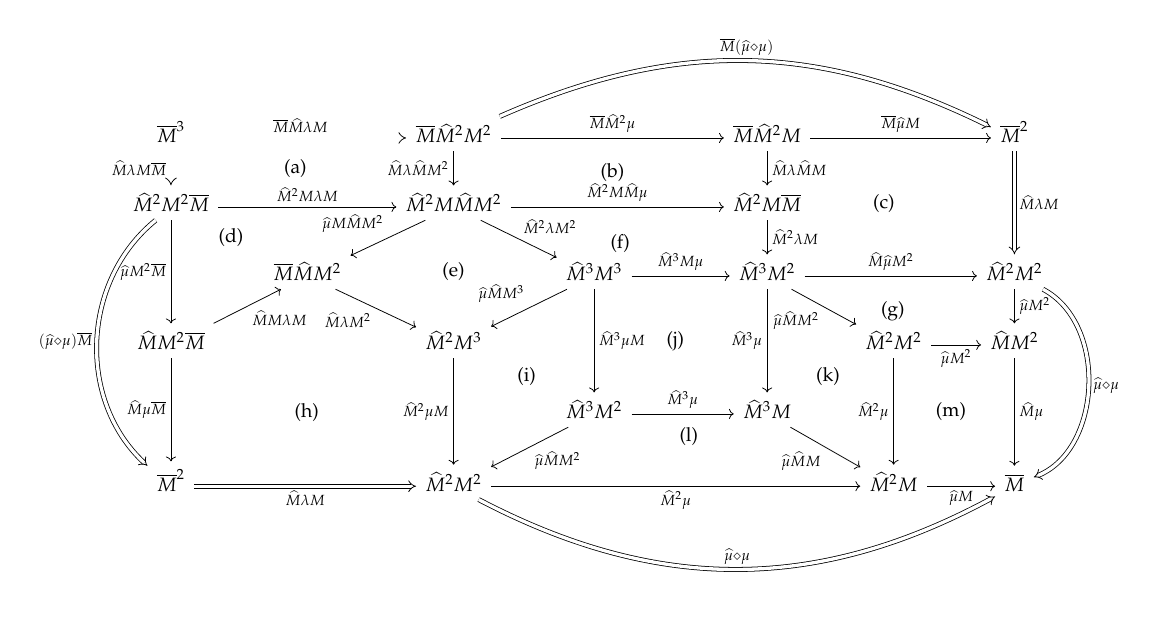
\begin{tikzpicture}[baseline= (a).base]
            \node[scale=.7] (a) at (0,0){
                \begin{tikzcd}
                    \overline{M}^3 \arrow[d, "\widehat{M}\lambda M\overline{M}"', Rightarrow] \arrow[rr, "\overline{M}\widehat{M}\lambda M", Rightarrow] \arrow[rrd, phantom, "\text{(a)}"] & & \overline{M}\widehat{M}^2M^2 \arrow[rrrrr, "\overline{M}(\widehat{\mu}\diamond \mu)", Rightarrow, bend left=25] \arrow[rrr, "\overline{M}\widehat{M}^2\mu"] \arrow[d, "\widehat{M}\lambda\widehat{M}M^2"'] \arrow[rrrd, phantom, "\text{(b)}"] & & & \overline{M}\widehat{M}^2M \arrow[rr, "\overline{M}\widehat{\mu}M"] \arrow[d, "\widehat{M}\lambda\widehat{M}M"] \arrow[rrdd, phantom, "\text{(c)}"] & & \overline{M}^2 \arrow[dd, "\widehat{M}\lambda M", Rightarrow] \\
                    \widehat{M}^2M^2\overline{M} \arrow[dddd, "(\widehat{\mu}\diamond \mu)\overline{M}"', Rightarrow, bend right=49] \arrow[dd, "\widehat{\mu}M^2\overline{M}"'] \arrow[rr, "\widehat{M}^2M\lambda M"] \arrow[rd, phantom, "\text{(d)}"] & & \widehat{M}^2M\widehat{M}M^2 \arrow[rrr, "\widehat{M}^2M\widehat{M}\mu"] \arrow[rd, "\widehat{M}^2\lambda M^2"] \arrow[ld, "\widehat{\mu}M\widehat{M}M^2"'] \arrow[dd, phantom, "\text{(e)}"] \arrow[rrrd, phantom, "\text{(f)}"] & & & \widehat{M}^2M\overline{M} \arrow[d, "\widehat{M}^2\lambda M"] & & \\
                    & \overline{M}\widehat{M}M^2 \arrow[rd, "\widehat{M}\lambda M^2"'] & & \widehat{M}^3M^3 \arrow[rr, "\widehat{M}^3M\mu"] \arrow[dd, "\widehat{M}^3\mu M"] \arrow[ld, "\widehat{\mu}\widehat{M}M^3"'] \arrow[lddd, phantom, "\text{(i)}"] \arrow[rrdd, phantom, "\text{(j)}"] & & \widehat{M}^3M^2 \arrow[rr, "\widehat{M}\widehat{\mu}M^2"] \arrow[rd, "\widehat{\mu}\widehat{M}M^2"'] \arrow[dd, "\widehat{M}^3\mu"'] \arrow[rrd, phantom, "\text{(g)}"] \arrow[rddd, phantom, "\text{(k)}"] & & \widehat{M}^2M^2 \arrow[d, "\widehat{\mu}M^2"] \arrow[ddd, "\widehat{\mu}\diamond \mu", Rightarrow, bend left=65] \\
                    \widehat{M}M^2\overline{M} \arrow[dd, "\widehat{M}\mu\overline{M}"'] \arrow[ru, "\widehat{M}M\lambda M"'] \arrow[rrdd, phantom, "\text{(h)}"] & & \widehat{M}^2M^3 \arrow[dd, "\widehat{M}^2\mu M"'] & & & & \widehat{M}^2M^2 \arrow[r, "\widehat{\mu}M^2"'] \arrow[dd, "\widehat{M}^2\mu"'] \arrow[rdd, phantom, "\text{(m)}"] & \widehat{M}M^2 \arrow[dd, "\widehat{M}\mu"] \\
                    & & & \widehat{M}^3M^2 \arrow[rr, "\widehat{M}^3\mu"] \arrow[ld, "\widehat{\mu}\widehat{M}M^2"] \arrow[rrrd, phantom, "\text{(l)}", near start] & & \widehat{M}^3M \arrow[rd, "\widehat{\mu}\widehat{M}M"'] & & \\
                    \overline{M}^2 \arrow[rr, "\widehat{M}\lambda M"', Rightarrow] & & \widehat{M}^2M^2 \arrow[rrrr, "\widehat{M}^2\mu"'] \arrow[rrrrr, "\widehat{\mu}\diamond\mu", Rightarrow, bend right=28] & & & & \widehat{M}^2M \arrow[r, "\widehat{\mu}M"'] & \overline{M} 
                \end{tikzcd}
            };
        \end{tikzpicture}
    \end{center}
    % \begin{equation}\label{diag-provingmultcomposite}
    
    % \end{equation}
    \begin{multicols}{2}
        \begin{enumerate}[(a)]
            \item Def of $\widehat{M}\lambda \diamond \lambda M$.
            \item Def of $\widehat{M}\lambda \widehat{M}\diamond \mu$.
            \item Apply $\widehat{M}(\cdot)M$ to \eqref{diag-mondistlaw2}.R.
            \item Def of $\widehat{\mu}\diamond M\lambda M$.
            \item Def of $\widehat{\mu}\diamond \lambda M^2$.
            \item Def of $\widehat{M}^2\lambda \diamond \mu$.
            \item Apply $(\cdot)M^2$ to associativity of $\widehat{\mu}$ \eqref{diag-multmonad}.
            \item Apply $\widehat{M}(\cdot)M$ to \eqref{diag-mondistlaw2}.L.
            \item Def of $\widehat{\mu}\widehat{M} \diamond \mu M$.
            \item Apply $\widehat{M}^3$ to associativity of $\mu$ \eqref{diag-multmonad}.
            \item Def of $\widehat{\mu}\widehat{M} \diamond \mu$.
            \item Same as (k): Def of $\widehat{\mu}\widehat{M} \diamond \mu$.
            \item Def of $\widehat{\mu} \diamond \mu$.
        \end{enumerate}
    \end{multicols}
\end{proof}
\begin{cor}\label{cor-Mp1monad}
    If $\mathbf{C}$ has (binary) coproducts and a terminal object $\mathbf{1}$ and $M$ is a monad, then $M(\cdot + \mathbf{1})$ is also monad.
\end{cor}
\begin{proof}
    We will exhibit a monad distributive law of $M$ over $(\cdot + \mathbf{1})$. We claim \[\iota_X : MX+\mathbf{1} \rightarrow M(X+1) = [M(\inl^{X+\mathbf{1}}), \eta_{X+\mathbf{1}} \circ \inr^{X+\mathbf{1}}]\]
    is a monad distributive law $\iota: (\cdot + \mathbf{1})M \Rightarrow M(\cdot +\mathbf{1})$. Then, it follows by Proposition \ref{prop-composemonad}.
\end{proof}
%Examples TODO: monoid and ring via term monads.
\begin{exmp}[Rings]
    Consider the term monads for the theory of monoids and abelian groups $T_{\textbf{Mon}}$ and $T_{\textbf{Ab}}$. You can check that they are the monads induced by the free-forgetful adjunctions between \textbf{Mon} and \textbf{Set} and \textbf{Ab} and \textbf{Set}. Also, $T_{\textbf{Mon}}$ is the same thing as the list monad. Call the binary operation of $T_{\textbf{Mon}}$ and $T_{\textbf{Ab}}$ the product and sum respectively.
    
    Then, by identifying products of sums (elements of $T_{\textbf{Mon}}T_{\textbf{Ab}}X$) with sums of products (elements of $T_{\textbf{Ab}}T_{\textbf{Mon}}X$) by \emph{distributing} the product over the sum as we are used to do with, say, real numbers, we obtain a monad distributive law of $T_{\textbf{Mon}}$ over $T_{\textbf{Ab}}$. The resulting composite monad $T_{\textbf{Ab}}T_{\textbf{Mon}}$ is the term monad for the theory of rings. The term distributive law comes from this example.
\end{exmp}
\begin{rem}
    It is not always possible to combine monads in such a natural way. For instance, it was shown that no distributive law exist between $\mPne$ and $\mathcal D$ and even that no monad structure can exist on $\mPne \mathcal D$ or $\mathcal D \mPne$. Thus, modelling combined probabilistic and nondeterministic effects has been quite a hard endeavor and is still an active area of research I discovered in an internship with Matteo Mio and Valeria Vignudelli at ENS de Lyon last summer.
\end{rem}
%Quickly : Generalized Determinization
If you are looking for more applications of this perspective on monads and especially if you enjoyed the assignment on Brzozowski's algorithm, I suggest you look into the paper \textit{Generalizing Determinization From Automata to Coalgebras} available at \url{https://arxiv.org/abs/1302.1046}.
\section{Exercises}
\begin{enumerate}
    \item Show that the triple $(\mathcal{D}, \eta, \mu)$ described in Example \ref{exmp-monads}.\ref{exmp-distmonad} is a monad.
    \item Show that the Kleisli category of the powerset monad is the category \textbf{Rel} of relations.
    \item Show that $\iota$ defined in the proof of Corollary \ref{cor-Mp1monad} is a monad distributive law.
    \item Show Proposition \ref{prop-Mp1} with the monad structure on $M(\cdot+\mathbf{1})$ given in Corollary \ref{cor-Mp1monad}.
\end{enumerate}

\end{document}

